% SPDX-License-Identifier: CC-BY-4.0
\section{Results}

\subsection{VLBI restores absolute station observability}

Take the default scenario first: 3 satellites, 6 Earth stations, seed 42. Adding
Earth-baseline VLBI pulls the recovered surface-station 3-D position error from
2183~m (range-only) down to 3.55~m, a factor of 615, and the satellite position
RMS from 717~m to 2.20~m. The fit converges in two iterations at a weighted RMS
residual of 0.05 over 40 observations and 16 parameters
(Figure~\ref{fig:headline}).

\begin{figure}[t]
  \centering
  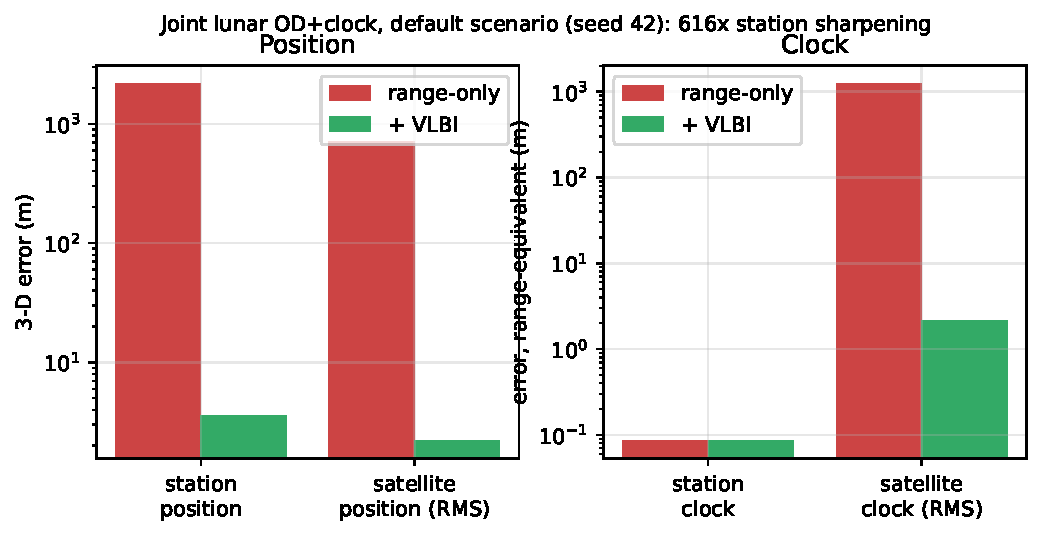
\includegraphics[width=\linewidth]{fig1_headline}
  \caption{With and without Earth-baseline VLBI in the default scenario
    (3 satellites, 6 Earth stations, seed 42). Left, position: VLBI sharpens the
    surface station's absolute 3-D error from 2183~m to 3.55~m ($615\times$) and
    the satellite position RMS from 717~m to 2.20~m. Right, clocks: the satellite
    clock RMS improves by about $569\times$, while the station clock, already
    pinned by the clock-sync pseudo-observable, barely moves (ratio 1.005).
    Modelled, internal-consistency oracle.}
  \label{fig:headline}
\end{figure}

That seed happens to be a favourable one. Over a 200-seed truth/noise ensemble
the median station error with VLBI is 13.4~m (IQR 5.9--23.0~m) against a
range-only median near 793~m, a median improvement of \textbf{91$\times$} (IQR
38--208$\times$; Figure~\ref{fig:seed_mc}). We quote the median, not the default
seed, which sits well into the upper tail. On a handful of seeds the factor is
close to one (the minimum over 200 is 0.91), so VLBI does not help on every
single draw, and we would rather say that than hide it.

The range-only regime is not a strawman. The first GNSS fix on the lunar surface
(LuGRE, 2025) worked at the tens-to-hundreds-of-metres level
\citep{lugre2026}, which is exactly where our range-only median of ~793~m lands.
Nor is the remedy hypothetical: the NovaMoon station ESA adopted at CM25 carries
an Earth-baseline VLBI transmitter of its own \citep{molli2026novamoon}, which
corroborates the design rationale this study isolates (it does not validate the
numbers).

\subsection{Information, not observation count}

If the observation set is held fixed and the VLBI delay $\sigma$ is degraded from
$10^{-12}$~s to $10^{-7}$~s, the median station error rises from 1.6~m to about
391~m and heads back toward the range-only median near 793~m
(Figure~\ref{fig:sigma_vlbi}). The extra observations are there the whole time;
only their information content changes. So the improvement is the VLBI
information, not the fifteen extra observations it brought with it. The default
$\sigma$, about 3~mm of delay precision and typical of geodetic VLBI, sits near
the informative end of the curve.

\begin{figure}[t]
  \centering
  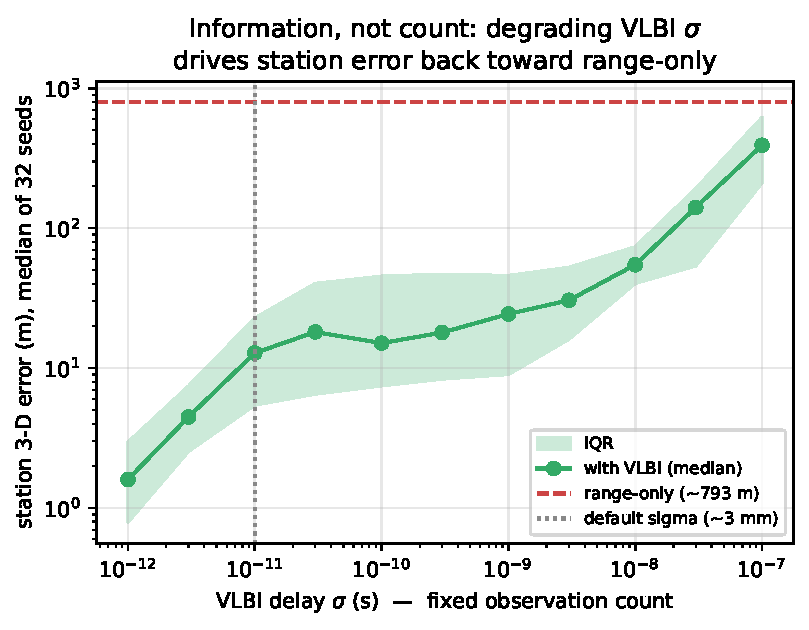
\includegraphics[width=0.8\linewidth]{fig2_sigma_vlbi}
  \caption{Information, not count. Median station 3-D error over a 32-seed
    ensemble as the VLBI delay $\sigma$ is degraded at fixed observation count.
    The error climbs from 1.6~m to about 391~m (with one minor non-monotonic step
    near $\sigma{=}10^{-10}$~s) and approaches the range-only median near 793~m:
    the observations stay, but their weight vanishes, so the gain was the VLBI
    information all along. The default $\sigma$ (~3~mm) sits near the informative
    end. Modelled.}
  \label{fig:sigma_vlbi}
\end{figure}

\subsection{The benefit is selective}

VLBI helps the absolute states and only those. In the default scenario the
satellite clock RMS improves by about $569\times$
($4.1\times10^{-6}$~s to $7.3\times10^{-9}$~s) alongside the position gains, but
the station clock error is essentially unchanged
($2.882\times10^{-10}$~s to $2.868\times10^{-10}$~s, ratio 1.005) because the
clock-sync pseudo-observable already pins it (Figure~\ref{fig:headline}, right).
VLBI is not a blanket improver. It supplies the absolute-geometry information the
lunar-local set is missing, and nothing it already has.

\subsection{The rank-restoration threshold, and the bound the estimator attains}

The minimum-baseline behaviour is not a soft conditioning effect; it is the
datum-defect closure of \S\ref{sec:theory} read straight off the Fisher
information. With one Earth station the joint network carries a six-dimensional
datum defect---the whole lunar frame floats---with two it is down to two, and at
three it is zero: full rank, absolute station position observable
(Figure~\ref{fig:n_earth}). Below three there is no finite Cram\'er--Rao bound and
the recovered error reflects the start point rather than an estimate, so we shade
that region.

Once the position is observable the bound sets the achievable accuracy. The
analytic Cram\'er--Rao bound on the station's absolute position falls from
\SI{50.1}{\meter} at three Earth stations to \SI{20.1}{\meter} at six and
\SI{13.7}{\meter} at ten---the diminishing-returns design curve of
Figure~\ref{fig:n_earth}---and the Gauss--Newton estimator's Monte-Carlo RMS
tracks it. At the default six-station network the two coincide: RMS
\SI{20.1}{\meter} against a bound of \SI{20.1}{\meter}, an efficiency of $1.00$
over 200 seeds. The estimator is statistically efficient---it extracts
essentially all the information the geometry holds---so the gains here are the
information-theoretic optimum, and a geodetic VLBI tie has a hard
minimum-infrastructure threshold that is not a margin you can trade away. (Right
at the threshold the 32-seed RMS sits a little under the bound; that is the
start-point regularisation biasing a marginally-conditioned solve, and it relaxes
by four stations.)

\begin{figure}[t]
  \centering
  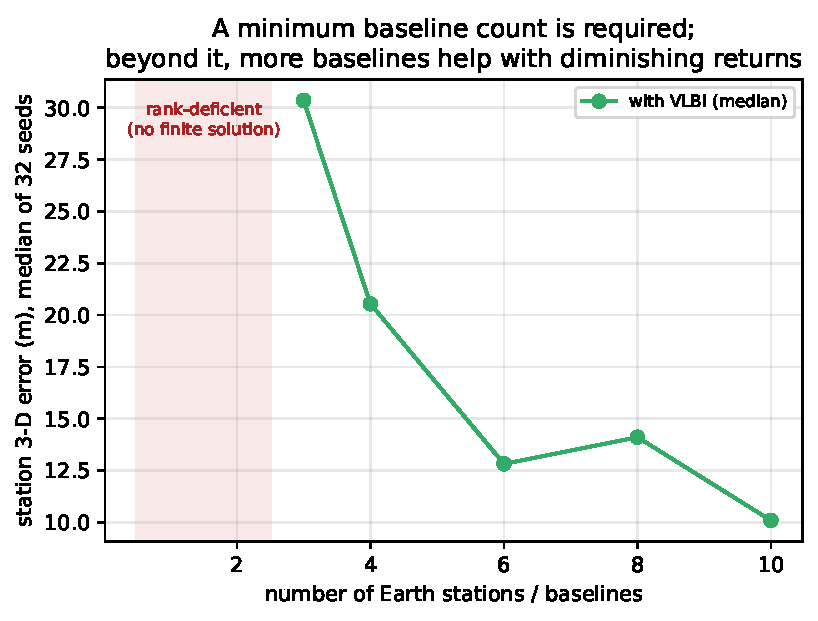
\includegraphics[width=0.8\linewidth]{fig3_n_earth}
  \caption{The rank-restoration threshold and the Cram\'er--Rao bound. With fewer
    than three Earth stations the Fisher information is rank-deficient (datum
    defect 6, then 2; shaded) and the absolute station position is unobservable;
    at three it becomes full rank. The analytic Cram\'er--Rao bound (line) then
    falls with baselines---\SI{50.1}{\meter} at three to \SI{13.7}{\meter} at
    ten---and the estimator's Monte-Carlo RMS (markers) tracks it, coinciding at
    the default six-station network (efficiency $1.00$). The FIM/CRLB engine is
    Validated against NumPy; the lunar network it is applied to is Modelled.}
  \label{fig:n_earth}
\end{figure}

\begin{figure}[t]
  \centering
  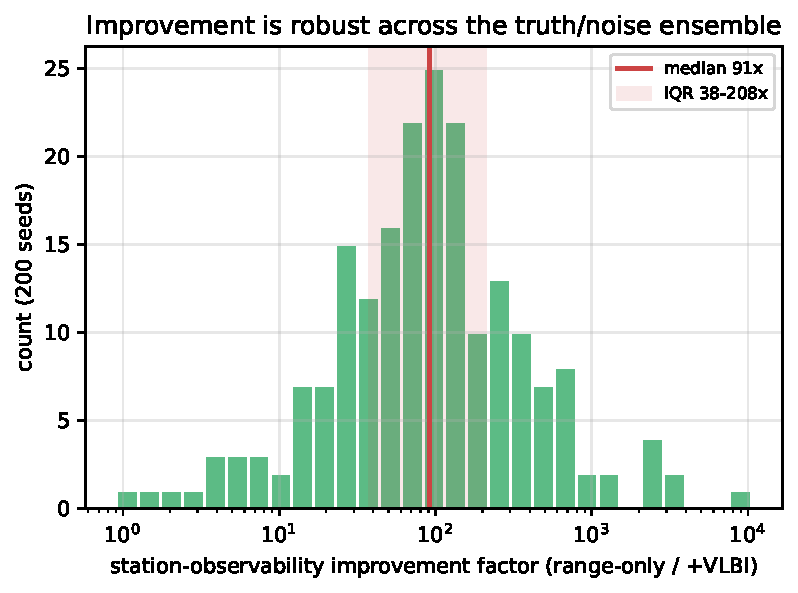
\includegraphics[width=0.8\linewidth]{fig4_seed_mc}
  \caption{Improvement factor over the 200-seed truth/noise ensemble (range-only
    over with-VLBI station 3-D error). The median is $91\times$ (IQR
    38--208$\times$); the with-VLBI median station error is 13.4~m (IQR
    5.9--23.0~m) against a range-only median near 793~m. The default seed
    ($615\times$) sits in the upper tail, and the minimum over 200 seeds is 0.91,
    so VLBI is not guaranteed to help on every draw. Modelled.}
  \label{fig:seed_mc}
\end{figure}

\subsection{Cross-suite sanity}

The same engine gives sensible numbers along the rest of the lunar chain
(Figure~\ref{fig:cross_suite}). Coordinated Lunar Time comes out at
57.04~$\mu$s/day \citep{ashby2024lunartime,iau2024lcrs}, split into a
$+57.50$~$\mu$s/day self-potential term and a $-0.46$~$\mu$s/day kinetic term.
That rate is Validated against Ashby \& Patla over DE440. It sits about
1~$\mu$s/day above their canonical surface-to-surface value of 56.02~$\mu$s/day,
and the difference is the choice of reference surface (Earth geoid versus lunar
selenoid potential), which is why the honest comparison is a band rather than a
point. The lunar-distance VLBI near-field correction is 58.9~$\mu$s on a
10\,727~km baseline, and its far-field limit reproduces the engine's own
far-field $\Delta$-DOR delay to machine precision (Modelled, against a
reference-implementation oracle in the same codebase). Differential PNT brings a
24.5~m standalone user error down to 0.008~m at a 50~km baseline ($3186\times$),
and the residual grows with baseline as you would expect (Modelled).

\begin{figure}[t]
  \centering
  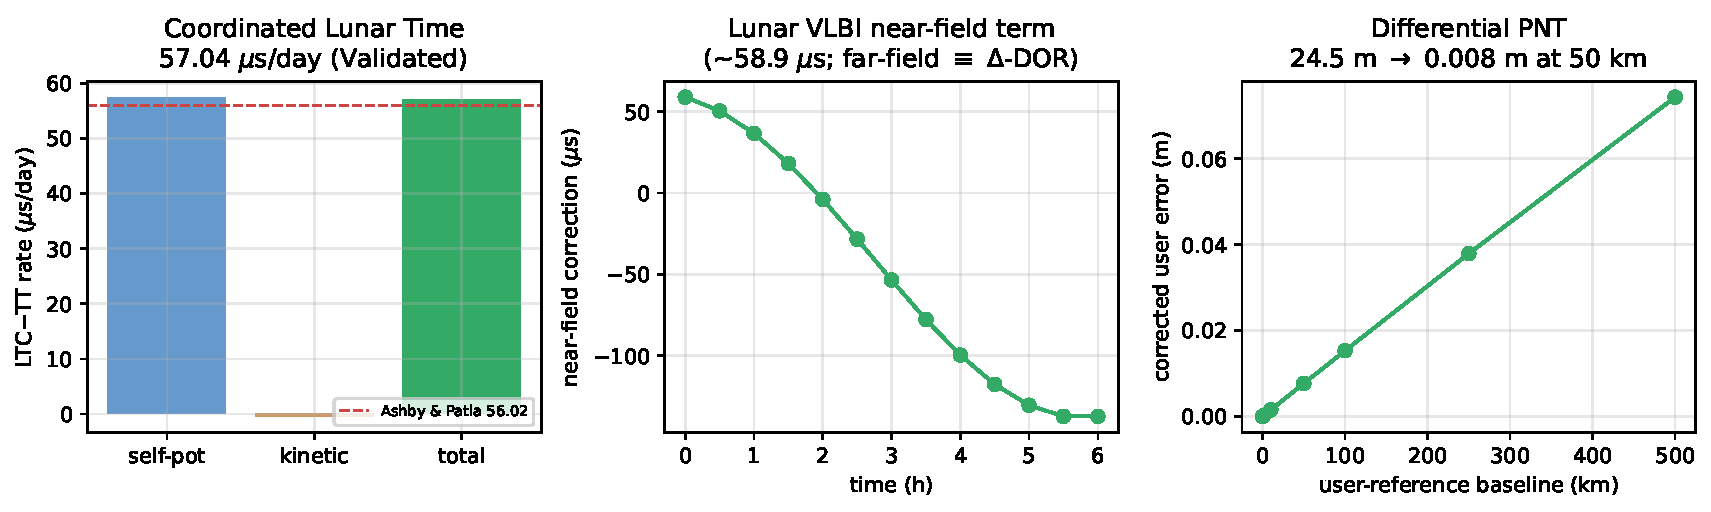
\includegraphics[width=\linewidth]{fig5_cross_suite}
  \caption{The same engine across the lunar chain. Left: Coordinated Lunar Time
    at 57.04~$\mu$s/day, split into a $+57.50$~$\mu$s/day self-potential term and
    a $-0.46$~$\mu$s/day kinetic term, Validated against Ashby \& Patla over DE440
    (the ~1~$\mu$s/day offset from their canonical 56.02~$\mu$s/day is the
    reference-surface choice). Centre: the lunar VLBI near-field correction,
    58.9~$\mu$s on a 10\,727~km baseline, whose far-field limit reproduces the
    engine's own far-field $\Delta$-DOR delay to machine precision (Modelled).
    Right: differential PNT taking a 24.5~m user error to 0.008~m at a 50~km
    baseline ($3186\times$), growing with baseline (Modelled).}
  \label{fig:cross_suite}
\end{figure}
